\section{Match hypothesis}

Our implementation considers a simple match algorithm(brute force). For each keypoints of frame $i$ we find the closest match in the frame $i+1$ iterating over all possible cantidates. We compare \textit{L2 Norm} and \textit{cosine} metrics to measure the similarity. Note that this implementation can generate the same match for two different keypoints yielding an outlier.

And idea of improvement of performance of this algorithm is to use \textit{KNN(K-Nearest Neighbors)}. For real time aplication this may be a good option because its complexity is $O(n\log n)$, while our approach is $O(n^2)$ ($n$ is the number of keypoints).

Figure \ref{fig:diff-l2-cosine} shows the different result comparing \textit{L2 Norm} and \textit{cosine} metrics.

\begin{figure}[!h]
	\centering
	\begin{subfigure}{0.5\textwidth}
	  \centering
	  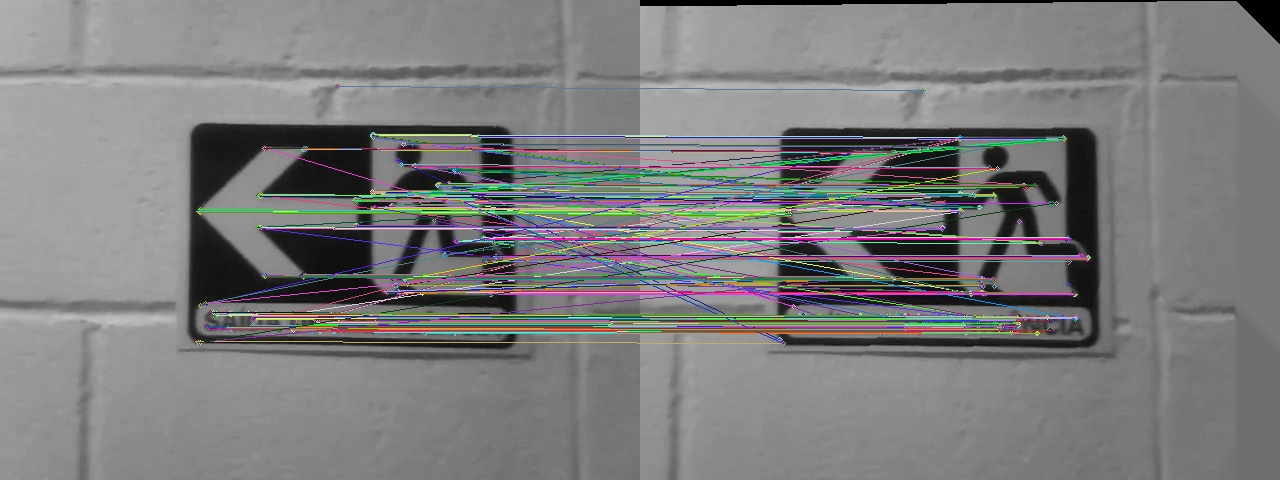
\includegraphics[width=0.8\linewidth]{figs/affine_100_cosine_30_8_False_p2-1-1_6-7.jpg}
	  \caption{Match hypotesis with cosine distance}
	\end{subfigure}%
	\begin{subfigure}{0.5\textwidth}
	  \centering
	  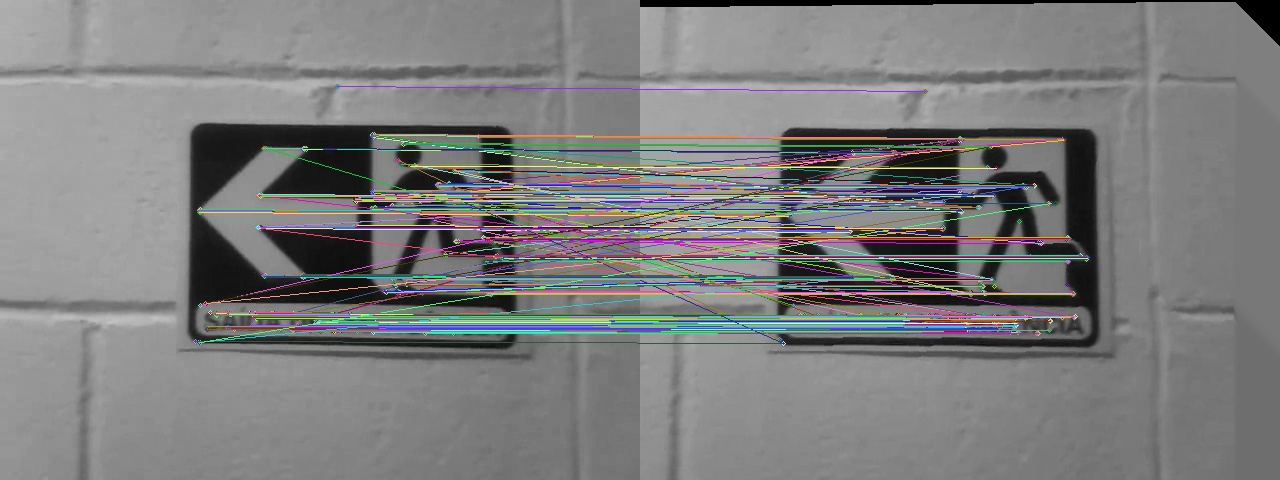
\includegraphics[width=0.8\linewidth]{figs/affine_200_l2-norm_30_8_False_p2-1-1_6-7.jpg}
	  \caption{Match hypotesis with l2-norm distance}
	\end{subfigure}
	\begin{subfigure}{0.5\textwidth}
        \centering
        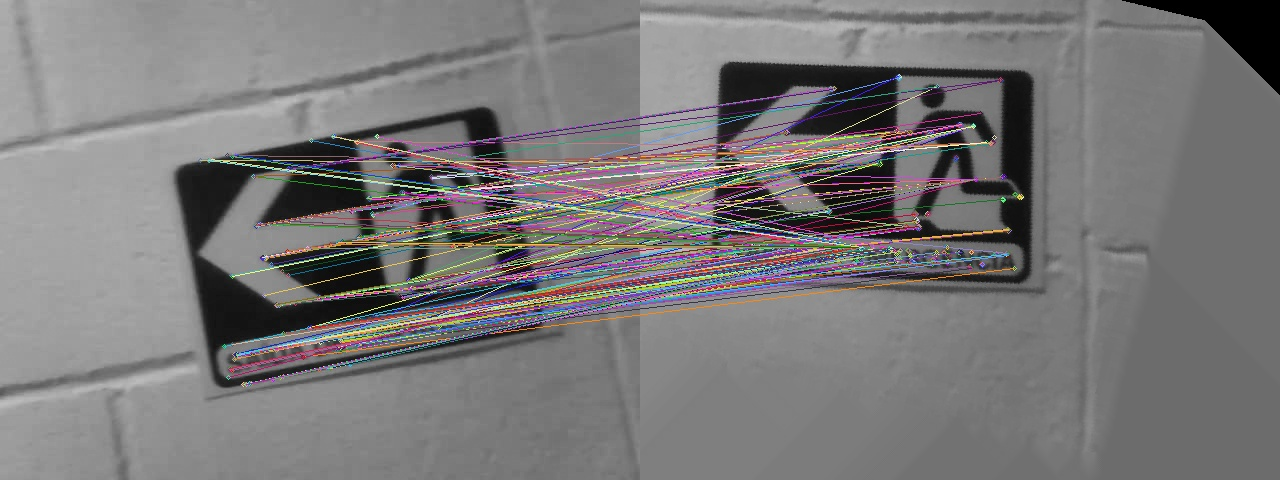
\includegraphics[width=0.8\linewidth]{figs/affine_100_cosine_30_8_False_p2-1-1_139-140.jpg}
        \caption{Match hypotesis with cosine distance}
      \end{subfigure}%
      \begin{subfigure}{0.5\textwidth}
        \centering
        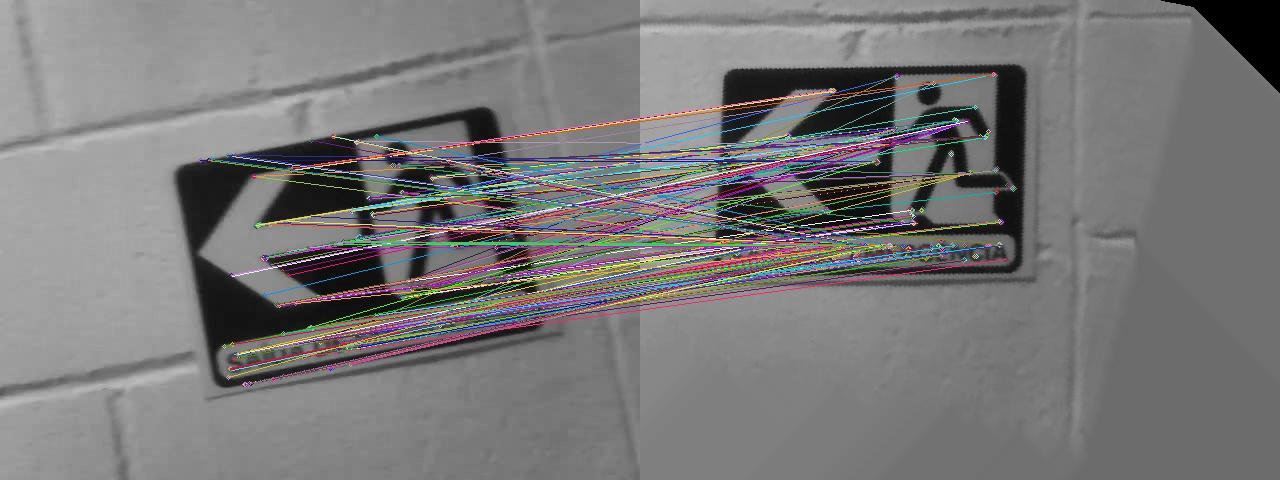
\includegraphics[width=0.8\linewidth]{figs/affine_200_l2-norm_30_8_False_p2-1-1_139-140.jpg}
        \caption{Match hypotesis with l2-norm distance}
      \end{subfigure}%
       \caption{Comparison of match hypothesis with cosine and l2-norm}
	\label{fig:diff-l2-cosine}
\end{figure}

